\chapter{Report}
\section{a}
The Relationships between Discharge and $\Delta S$ is shown in \autoref{fig:relationship}.
\begin{figure}[htpb]\centering
	\subfigure[]{
		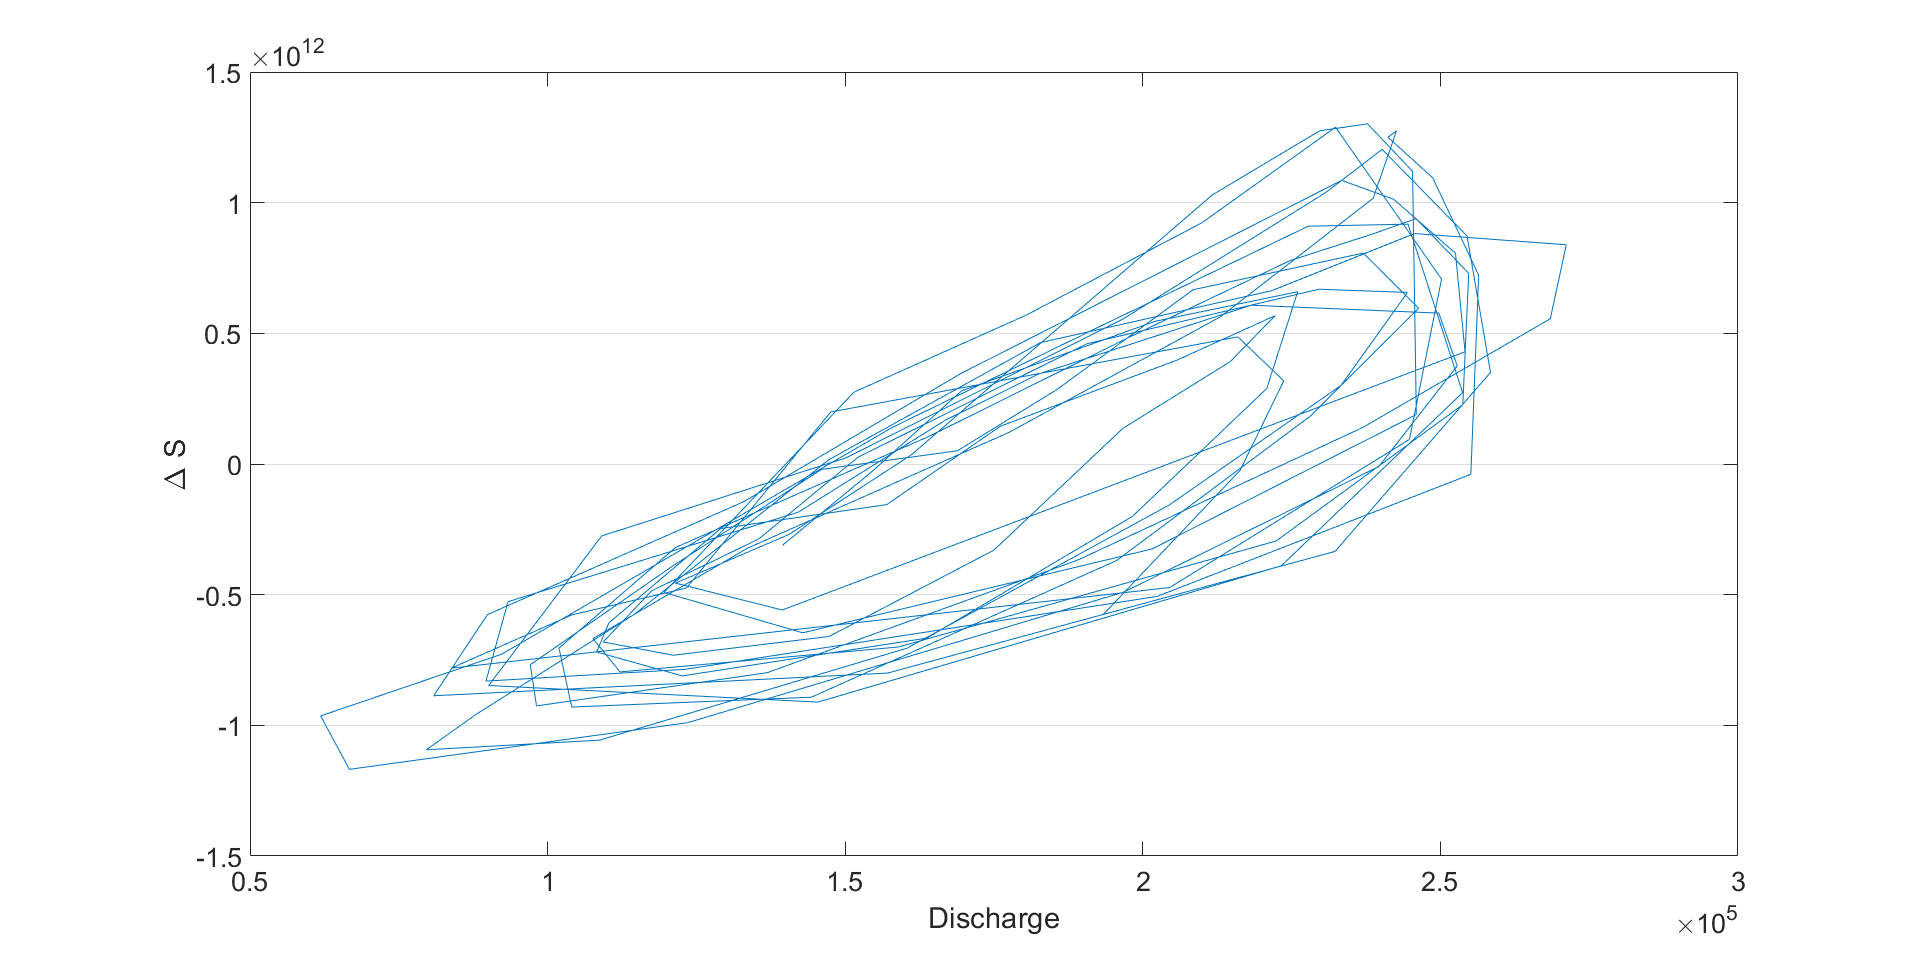
\includegraphics[width=0.9\textwidth]{relationship.png}}
	\caption{}
	\label{fig:relationship}
\end{figure}
\section{b}
\begin{equation*}
	\frac{dR}{dt} + \frac{R}{\tau} = \omega^2_n S
\end{equation*}
\section{c}
\begin{gather*}
	\frac{R_t - R_{t-1}}{\Delta t} + \frac{R_t}{\tau} = \omega^2_n S_t \\
\end{gather*}
If we take $\Delta t$ as 1 unit.
\begin{gather*}
	R_t - R_{t-1} + \frac{R_t}{\tau} = \omega^2_n S_t \\
	\left(1+\frac{1}{\tau}\right) R_{t} = R_{t-1} +  \omega^2_n S_t \\
	R_{t} = \frac{\tau}{\tau + 1} R_{t-1} + \frac{\tau \omega_n^2}{\tau + 1}S_t
\end{gather*}
\section{d}
\begin{align*}
	R_{t} = & \frac{\tau}{\tau + 1} R_{t-1} + \frac{\tau \omega_n^2}{\tau + 1}S_t \\
		  = & \frac{\tau}{\tau + 1} R_{t-1} + \frac{\tau \omega_n^2}{\tau + 1}S_0 + \frac{\tau \omega_n^2}{\tau + 1} \sum_{i=1}^{t} \Delta S_i \\
		  = & \alpha R_{t-1} + \beta + \gamma \sum_{i=1}^{t} \Delta S_i
\end{align*}
Thus we have:
\begin{gather*}
	S_0 = \frac{\beta}{\gamma} \\
	\omega_0 = \sqrt{\frac{\gamma}{\alpha}} \\
	\tau = \frac{\alpha}{1-\alpha}
\end{gather*}
The 3 parameters can be calculated using least square since we have discharge and $\Delta S$ data.
\clearpage
\begin{gather*}
	R(t) = R(t-1)e^{\frac{\Delta t}{\tau}} + e^{\frac{\Delta t}{\tau}} \omega^2 \int S(t) e^{\frac{-\Delta t}{\tau}} dt \\
	R(t) = R(t-1)e^{\frac{\Delta t}{\tau}} +  \omega^2\left[\frac{S(t-1) + S(t)}{2} \cdot \Delta t\right]
\end{gather*}\\\\\\\\

\begin{gather*}
	\omega^2 \tau (e^{\frac{\Delta t}{\tau}} - 1) \\
	R(t_{n+1}) = R(t_{n}) e^{\frac{\Delta t}{\tau}} + \bar{S}(t_{n}) \cdot \omega^2 \tau (e^{\frac{\Delta t}{\tau}} - 1) \\
	R(t_{n+1}) = R(t_{n}) e^{\frac{\Delta t}{\tau}} + \left(S_0 + \Delta S(t_{n})\right) \cdot \omega^2 \tau (e^{\frac{\Delta t}{\tau}} - 1)
\end{gather*}
before from CSR, after GPL